\iffalse
\chapter{2007}
\author{AI24BTECH11020}
\section{ce}
\fi

%\begin{enumerate}[start=18]
	\item The consistency and flow resistance of bitumen can be determined from the following:
	\begin{enumerate}
		\item Ductitility test
		\item Penetration test
		\item Softening point test
		\item Viscosity test
	\end{enumerate}
\item If a two-lane national highway and a two-lane state highway intersect at right angles, the number of potential conflict points at the intersection, assuming that both the roads are two-way is 
	\begin{enumerate}
                \item $11$
                \item $17$
		\item $24$
                \item $32$
        \end{enumerate}
\item In signal design as per Indian Roads Congress specifications, if the sum of the ratios of normal flows to saturation flow of two directional traffic flow is $0.50$ and the total lost time per cycle is $10$ seconds, the optimum cycle length in seconds is 
	\begin{enumerate}
                \item $100$
                \item $80$
                \item $60$
                \item $40$
        \end{enumerate}
		\section*{Q.21 to Q.75 carry two marks each.}
\item For what values of $\alpha$ and $\beta$ the following simultaneous equations have an infinite number of solutions?\\ $x+y+z=5;  x+3y+3z=9;  x+2y+\alpha z= \beta$
	\begin{enumerate}
                \item $2,7$
                \item $3,8$
                \item $8,3$
                \item $7,2$
        \end{enumerate}
\item A velocity vector is given as $\vec{V}= 5xy\overrightarrow{i}+2y^2\overrightarrow{j}+3yz^2\overrightarrow{k}$. The divergence of this velocity vector at $\brak{1,1,1}$ is
	\begin{enumerate}
                \item $9$
                \item $10$
                \item $14$
                \item $15$
        \end{enumerate}
\item A body originally at $60{\degree}C$ cools down to $40{\degree}C$ in $15$ minutes when kept in air at a temperature of $25{\degree}C$. what will be the temperature of the body at the end of $30$ minutes?
	\begin{enumerate}
		\item $35.2{\degree}C$
                \item $31.5{\degree}C$
                \item $28.7{\degree}C$
                \item $15{\degree}C$
        \end{enumerate}
\item The following equation needs to be numerically solved using the Newton-Raphson method.\\ $$x^3+4x-9=0$$\\The iterative equation for this purpose is ($k$ indicates the iteration level)
	\begin{enumerate}
		\item $x_{k+1}=\frac{2x_k^3+9}{3x_k^2+4}$
		\item $x_{k+1}=\frac{3x_k^2+4}{2x_k^2+9}$
		\item $x_{k+1}=x_k-3x_k^2+4$
		\item $x_{k+1}=\frac{4x_k^2+3}{9x_k^2+2}$
        \end{enumerate}   
\item Evaluate $\int\limits_{0}^{\infty} \frac{\sin t}{t} dt$
	\begin{enumerate}
                \item $\pi$
		\item $\frac{\pi}{2}$
		\item $\frac{\pi}{4}$
		\item $\frac{\pi}{8}$  
        \end{enumerate}
\item Potential function $\phi$ is given as $\phi=x^2-y^2$. What will be the stream function$(\psi)$ with the condition $\psi=0$ at $x=y=0$?
	\begin{enumerate}
                \item $2xy$
                \item $x^2+y^2$
                \item $x^2-y^2$
                \item $2x^2y^2$  
        \end{enumerate}
\item The inverse of the $2 \times 2$  matrix $\myvec{1 & 2 \\ 5 & 7}$  is,
\begin{enumerate}
	\item $\frac{1}{3} \myvec{ -7 & 2 \\ 5 & -1 }$\\
\item $ \frac{1}{3} \myvec{7 & 2 \\ 5 & 1}$\\
\item $\frac{1}{3} \myvec{7 & -2 \\ -5 & 1}$\\
\item $\frac{1}{3} \myvec{-7 & -2 \\ -5 & -1}$\\
		\end{enumerate}
\item Given that one root of the equation $x^3-10x^2+31x-30=0$ is $5$, the other two roots are
\begin{enumerate}
                \item $2$ and $3$
                \item $2$ and $4$
                \item $3$ and $4$
                \item $-2$ and $-3$
        \end{enumerate}
\item If the standard deviation of the spot speed of vehicles in a highway is $8.8 kmph$ and the mean speed of the vehicles is $33 kmph$, the coefficient of variation in speed is 
	\begin{enumerate}
                \item $0.1517$
                \item $0.1867$
                \item $0.2666$
                \item $0.3646$
        \end{enumerate}
\item A metal bar of length $100 mm$ is inserted between two rigid supports and its temperature is increased by $10{\degree}C$. If the coefficient of thermal expansion is $12 \times 10^{-6}$ per ${\degree}C$ and the Young's modulus is $2 \times 10^5 MPa$, the stress in the bar is 
	\begin{enumerate}
                \item zero
                \item $12 MPa$
                \item $24 MPa$
                \item $2400 MPa$
        \end{enumerate}
\item A rigid bar is suspended by three rods made of the same material as shown in the figure. The area and length of the central rod are $3A$ and $L$, respectively while that of the two outer rods are $2A$ and $2L$,respectively. If a downward force of $50 kN$ is applied to the right bar, the forces in the central and each of the outer rods will be\\
	\begin{center}	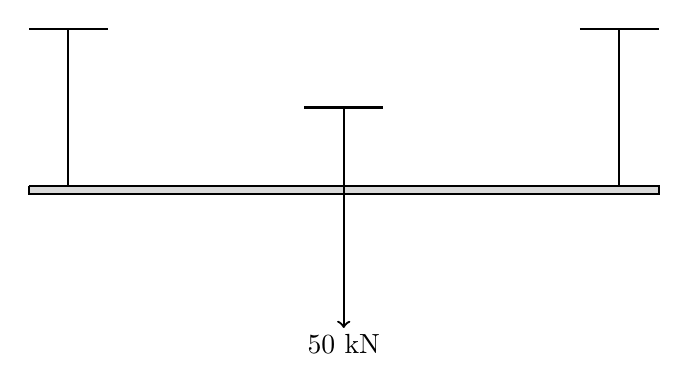
\begin{tikzpicture}
		\draw[thick, fill=gray!30](-4,0) -- (4,0) -- (4,-0.1) -- (-4,-0.1) -- (-4,0);
    \draw[thick] (-3.5, 0) -- (-3.5, 2) -- (-4, 2);
    \draw[thick] (-3.5, 2) -- (-3, 2); 
    \draw[thick] (3.5, 0) -- (3.5, 2) -- (4, 2);
    \draw[thick] (3, 2) -- (3.5, 2); 
    \draw[thick] (0, 0) -- (0, 1) -- (-0.5, 1);
    \draw[thick] (0, 1) -- (0.5, 1);
    \draw[thick, ->] (0, 0) -- (0, -1.8);
    \node at (0, -2) {50 kN}; 
	\end{tikzpicture} \end{center}
		\begin{enumerate}
                \item $16.67 kN$ each
                \item $30 kN$ and $15 kN$
                \item $30 kN$ and $10 kN$
                \item $21.4 kN$ and $14.3 kN$
        \end{enumerate}
\item The maximum and minimum shear stresses in a hollow circular shaft of outer diameter $20 mm$ and thickness $2 mm$, subjected to a torque of $92.7 N.m$ will be
	\begin{enumerate}
                \item $59 MPa$ and $47.2MPa$
                \item $100 MPa$ and $80 MPa$
                \item $118 MPa$ and $160 MPa$
                \item $200 MPa$ and $160 Mpa$
        \end{enumerate}
\item The shear stress at the neutral axis in a beam of triangular section with a base of $40 mm$ and height $20 mm$, subjected to a shear force of $34 kN$ is
	\begin{enumerate}
                \item $3 MPa$
                \item $6 MPa$
                \item $10 MPa$
                \item $20 MPa$
        \end{enumerate}
\item $U_1$ and $U_2$ are the strain energies stored in a prismatic bar due to axial tensile forces $P_1$ and $P_2$,respectively. The strain energy $U$ stored in the same bar due to combined action of $P_1$ and $P_2$ will be 
\begin{enumerate}
                \item $U=U_1+U_2$
                \item $U=U_1U_2$ 
                \item $U<U_1+U_2$ 
                \item $U>U_1+U_2$ 
        \end{enumerate}     

%\end{enumerate}
 

